\section{NextDAO}
\subsection{区块链协作}
以太坊ERC20的出现,以区块链智能合约技术为基础,成为了一种新型、快捷、低成本的融资方式,但融资过后的协作和管理问题并没有得到很好的解决。这一直都是区块链重要的发展方向之一,并同时带来了很多问题。

The DAO(Decentralized Autonomous Organization)~\cite{DAO},又叫“去中心化自治组织”一个以公开透明的计算机代码来体现的组织,其受控于股东,并不受中心化组织影响。The DAO发布之后,很快被黑客攻击并盗走价值千万美金价值的以太坊,最终导致以太坊硬分叉。虽然The DAO存在着缺陷,但给后续的工作带来了很多借鉴的作用。

星云链致力于区块链协作的发展,并在此基础上提出了基于区块钱链协作的框架范式集合:NextDAO。具体包含:公链协作、治理、去中心化金融(DeFi)等,详细如图\ref{fig:nextdao}所示。NextDAO尝试着解决目前区块链的协作当中存在的几个问题:

\begin{enumerate}[\hspace{1cm}(a)]
  \item 激励方式仍以出块奖励为主
  \item 公平与正向博弈缺失
  \item 协作方式单一
\end{enumerate}

\begin{figure}[htbp]
  \centering
  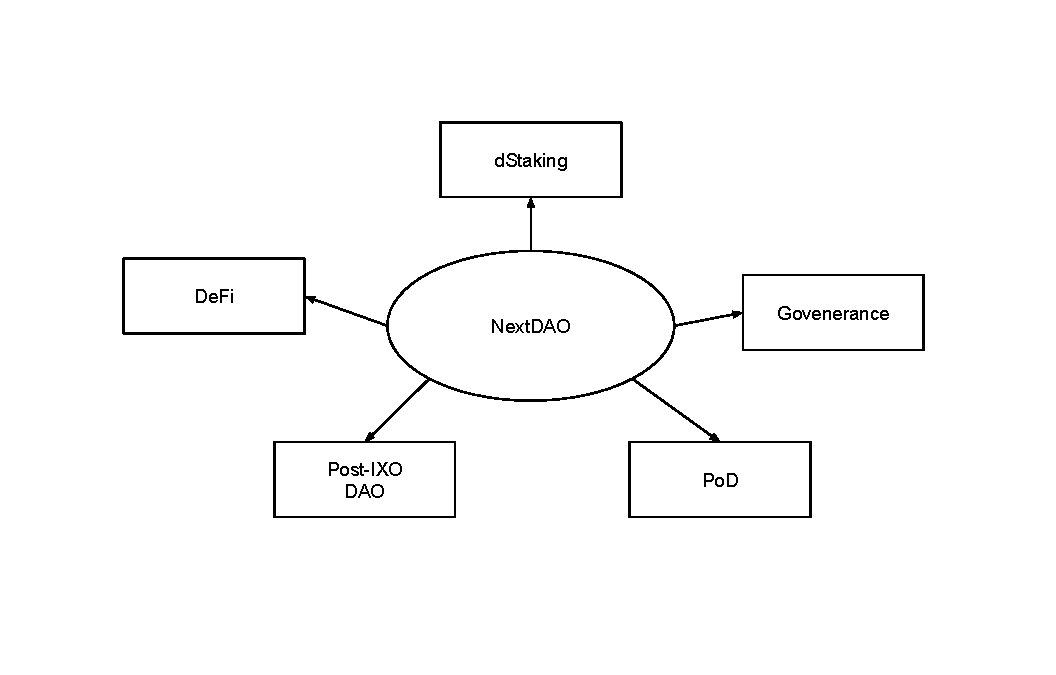
\includegraphics[width=1\textwidth]{../common/nextdao.pdf}
  \caption{区块链协作范式集合:NextDAO \label{fig:nextdao}}
\end{figure}

\subsection{公链通证经济}
通证经济(Token Economy),具体表现为包含通证产生、流通、回购、激励的经济模型。通证经济存在于区块链世界各个角落,例如公链生态、DApp应用内部等。公链生态通证经济的典型的案例是以太坊的ERC20,它便利了融资的同时,刺激和繁荣了以太坊生态,也同时带动了整个区块链行业的大发展。因此,公链的价值和创新不仅仅源于在“不可能的三角”上的技术本身的创新,也来源于技术所带来的模式和商业创新。

公链通证经济要考虑的问题是人与人的博弈,需要避免公地悲剧~\cite{TragedyOfTheCommons},通过正向激励促进公链生态的繁荣和发展。大多数公链远达不到以太坊的社区力量,因此以探索区块链应用落地为导向,发展区块链技术,扩大社区共识,才能建立一个适合自身的优秀的公链通证经济,这与发展公链技术创新同等重要。接下来的章节,将详细介绍星云链根据自身的愿景和特点,提出来的基于NextDAO框架的公链通证范式:NAX。
